\documentclass{beamer}
\usepackage{lmodern}

\usepackage{xeCJK}

\usepackage[safe]{silence}
\WarningFilter*{latexfont}{Font}

\usetheme{CambridgeUS} % try Madrid, Pittsburgh
\usecolortheme{beaver}
\usefonttheme[onlymath]{serif} % try "professionalfonts"

\setbeamertemplate{itemize items}[default]
\setbeamertemplate{enumerate items}[default]

\usepackage{amsmath, amsfonts, latexsym, mathtools}
% \usepackage{kbordermatrix}
% \usepackage{ntheorem}

\usepackage{centernot}

\DeclareMathOperator*{\argmin}{arg\,min}
\DeclareMathOperator*{\argmax}{arg\,max}

% colors
\newcommand{\red}[1]{\textcolor{red}{#1}}
\newcommand{\green}[1]{\textcolor{green}{#1}}
\newcommand{\blue}[1]{\textcolor{blue}{#1}}
\newcommand{\purple}[1]{\textcolor{purple}{#1}}

% colorded box
\newcommand{\rbox}[1]{\red{\boxed{#1}}}
\newcommand{\gbox}[1]{\green{\boxed{#1}}}
\newcommand{\bbox}[1]{\blue{\boxed{#1}}}
\newcommand{\pbox}[1]{\purple{\boxed{#1}}}

\usepackage{tikz}
% see http://tex.stackexchange.com/a/7045/23098
\newcommand*\circled[1]{\tikz[baseline=(char.base)]{
            \node[shape=circle,draw,inner sep=2pt] (char) {#1};}}
\usepackage{tikz-qtree}
\usetikzlibrary{backgrounds, fit}

\usepackage{pifont}
\usepackage{wasysym}

\usepackage[normalem]{ulem}
\newcommand{\middlewave}[1]{\raisebox{0.5em}{\uwave{\hspace{#1}}}}

\usepackage{graphicx, subcaption}

\usepackage{algorithm}
\usepackage[noend]{algpseudocode}

\newcommand{\pno}[1]{\textcolor{blue}{\scriptsize [Problem: #1]}}
\newcommand{\set}[1]{\{#1\}}
\DeclareMathOperator{\lcm}{lcm}

\newcommand{\cmark}{\green{\ding{51}}}
\newcommand{\xmark}{\red{\ding{55}}}
%%%%%%%%%%%%%%%%%%%%%%%%%%%%%%%%%%%%%%%%%%%%%%%%%%%%%%%%%%%%%%
% for fig without caption: #1: width/size; #2: fig file
\newcommand{\fignocaption}[2]{
  \begin{figure}[htp]
    \centering
      \includegraphics[#1]{#2}
  \end{figure}
}

% for fig with caption: #1: width/size; #2: fig file; #3: fig caption
\newcommand{\fig}[3]{
  \begin{figure}[htp]
    \centering
      \includegraphics[#1]{#2}
      \caption[labelInTOC]{#3}
  \end{figure}
}

\newcommand{\titletext}{Number-Theoretic Algorithms}
%%%%%%%%%%%%%%%%%%%%
\title[\titletext]{\titletext}
\subtitle{}

\author[Hengfeng Wei]{Hengfeng Wei}
\institute{hfwei@nju.edu.cn}
\date{March 31 $\sim$ \today}

\AtBeginSection[]{
  \begin{frame}[noframenumbering, plain]
    \frametitle{\titletext}
    \tableofcontents[currentsection, sectionstyle=show/shaded, subsectionstyle=show/show/hide]
  \end{frame}
}
%%%%%%%%%%
\begin{document}
\maketitle

\section{Modular Arithmetic}

\begin{frame}{``Mod''}
  \begin{exampleblock}{(TC 31.4.2)}
	\[
	  ad \equiv bd \pmod{n}, \textcolor{red}{a \bot n} \implies a \equiv b \pmod{n} 
	\]
  \end{exampleblock}

  \[
	3 \cdot 2 \equiv 5 \cdot 2 \pmod{4} \quad \textcolor{red}{3 \not\equiv 5 \pmod{4}} \quad \pause \textcolor{blue}{3 \equiv 5 \pmod{2}}
  \]
\end{frame}
%%%%%%%%%%%%%%%%%%%%
\begin{frame}{Changing the modulus}
  \[
	ad \equiv bd \pmod{nd} \iff a \equiv b \pmod{n} \quad (d \neq 0)
  \]

  \[
	ad \equiv bd \pmod{n} \iff a \equiv b \pmod{\frac{n}{\gcd(d,n)}}
  \]
\end{frame}
%%%%%%%%%%%%%%%%%%%%
\begin{frame}{Changing the modulus}
  \[
	a \equiv b \pmod{100} \implies a \equiv b \pmod{20} \implies a \equiv b \pmod{5}
  \]

  \[
	a \equiv b \pmod{nd} \implies a \equiv b \pmod{n}, d \in \mathbb{Z}
  \]

  \centerline{\rule{0.80\paperwidth}{0.4pt}}

  \[
	a \equiv b \pmod{n_1}, a \equiv b \pmod{n_2} \iff a \equiv b \pmod{\lcm(n_1, n_2)}
  \]

  % \[
  %   a \equiv b \pmod{12}, a \equiv b \pmod{18} \iff a \equiv b \pmod{36}
  % \]

  \[
	a \equiv b \pmod{n_1}, a \equiv b \pmod{n_2} \iff a \equiv b \pmod{n_1n_2}, \text{ if } n_1 \bot n_2
  \]

  \[
	a \equiv b \pmod{n} \iff a \equiv b \pmod{p^{n_p}}, \quad n = \prod_{p} p^{n_p}
  \]
\end{frame}
%%%%%%%%%%%%%%%%%%%%
\begin{frame}{Changing the modulus}
\end{frame}
%%%%%%%%%%%%%%%%%%%%
%%%%%%%%%%%%%%%%%%%%


\section{Euclid's GCD Algorithm}

%%%%%%%%%%%%%%%%%%%%
%%%%%%%%%%%%%%%%%%%%
%%%%%%%%%%%%%%%%%%%%
%%%%%%%%%%%%%%%%%%%%
%%%%%%%%%%%%%%%%%%%%
%%%%%%%%%%%%%%%%%%%%
%%%%%%%%%%%%%%%%%%%%
%%%%%%%%%%%%%%%%%%%%

\section{Pairwise Relatively Prime}

%%%%%%%%%%%%%%%%%%%%
\begin{frame}{Pairwise relatively prime}
  \begin{exampleblock}{(TC 31.2--9)}
	\begin{gather*}
	  n_1, n_2, n_3, n_4 \text{ are pairwise relatively prime} \\
	  \iff \\
	  \gcd(n_1n_2, n_3n_4) = \gcd(n_1n_3, n_2n_4) = 1
	\end{gather*}
  \end{exampleblock}
\end{frame}
%%%%%%%%%%%%%%%%%%%%
\begin{frame}{Pairwise relatively prime}
  \begin{exampleblock}{(TC 31.2--9)}
	\begin{gather*}
	  n_1, n_2, \dots, n_k \text{ are pairwise relatively prime} \\
	  \iff \\
	  \text{a set of } \lceil \lg k \rceil \text{ pairs of numbers derived from the } n_i \text{ are relatively prime}.
	\end{gather*}
  \end{exampleblock}

  \pause
  \[
	\binom{k}{2} = \Theta(k^2)	\quad (\text{complete graph})
  \]

  \pause
  \[
	\textcolor{red}{\gcd(\fbox{$1_L$}, \fbox{$1_R$}) 
	= \gcd(\fbox{$2_L$}, \fbox{$2_R$}) 
	= \cdots 
	= \gcd(\fbox{$\lceil \lg k \rceil_L$}, \fbox{$\lceil \lg k \rceil_R$}) = 1}
  \]

  \pause
  \begin{gather*}
	k = 3: \quad \gcd(n_1, n_2n_3) = \gcd(n_2, n_3) = 1 \\
	k = 2: \quad \gcd(n_1, n_2) = 1
  \end{gather*}
\end{frame}
%%%%%%%%%%%%%%%%%%%%
\begin{frame}{Pairwise relatively prime: divide-and-conquer}
  % \begin{center}
  %     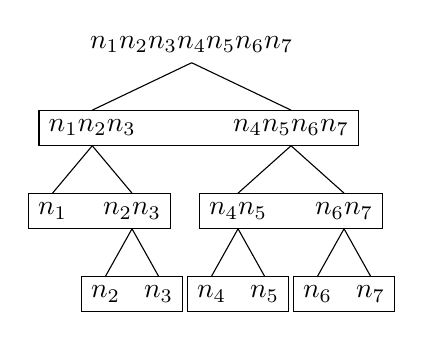
\begin{tikzpicture}
	\Tree [.\node (1234567) {$n_1n_2n_3n_4n_5n_6n_7$};
	  [.\node (123) {$n_1n_2n_3$};
		[.\node (1) {$n_1$}; ] 
		  [.\node (23) {$n_2n_3$};
			[.\node (2) {$n_2$}; ]
			[.\node (3) {$n_3$}; ]]] 
	  [.\node (4567) {$n_4n_5n_6n_7$};
		[.\node (45) {$n_4n_5$};
		  [.\node (4) {$n_4$}; ] 
		  [.\node (5) {$n_5$}; ]]
		[.\node (67) {$n_6n_7$};
		  [.\node (6) {$n_6$}; ] 
		  [.\node (7) {$n_7$}; ]]]]

	\begin{pgfonlayer}{background}
	  % \node () [ellipse, draw, fit = (1234567), inner sep = 0pt] {};
	  \pause
	  \node () [rectangle, draw, fit = (2) (3), inner sep = 0pt] {};
	  \node () [rectangle, draw, fit = (4) (5), inner sep = 0pt] {};
	  \node () [rectangle, draw, fit = (6) (7), inner sep = 0pt] {};
	  \node () [rectangle, draw, fit = (1) (23), inner sep = 0pt] {};
	  \node () [rectangle, draw, fit = (45) (67), inner sep = 0pt] {};
	  \node () [rectangle, draw, fit = (123) (4567), inner sep = 0pt] {};
	\end{pgfonlayer}
  \end{tikzpicture}

  % \end{center}

  \fignocaption{width = 0.40\textwidth}{figs/coprime7.pdf}

  \pause
  \begin{equation*}
	\begin{cases}
	  T(1) = 0 \\
	  T(k) = 2T(\frac{k}{2}) + 1
	\end{cases} \pause \implies T(k) = k - 1
  \end{equation*}

  \pause
  \[
	T_k = k-1: (n_i, n_{i+1}n_{i+2}\cdots n_{k}) \quad \forall 1 \le i < k
  \]
\end{frame}
%%%%%%%%%%%%%%%%%%%%
\begin{frame}{Pairwise relatively prime: smarter combination}
  \begin{equation*}
	\begin{cases}
	  T(1) = 0 \\
	  T(k) = T(\frac{k}{2}) + 1
	\end{cases}\pause \implies T(k) = \lceil \lg k \rceil
  \end{equation*}
\end{frame}
%%%%%%%%%%%%%%%%%%%%
\begin{frame}{Pairwise relatively prime: the dividing pattern}
  \[
	k = 7: \quad n_{\textcolor{red}{0}}, n_1, n_2, \ldots, n_6
  \]

  \begin{gather*}
	000\\
	001\\
	010\\
	011\\
	100\\
	101\\
	110
  \end{gather*}

  \pause
  \[
	T(k) = \lceil \lg k \rceil
  \]
\end{frame}
%%%%%%%%%%%%%%%%%%%%
\begin{frame}{Can we do even better?}
  \[
	T(k) \ge \lceil \lg k \rceil
  \]

  \pause
  \centerline{Prove by (strong) mathematical induction.}

  \pause
  \begin{align*}
	T(k) &\ge 1 + T(\lceil \frac{k}{2} \rceil) \\
		&\ge 1 + \lceil \lg \lceil \frac{k}{2} \rceil \rceil \\
		&= \lceil \lg k \rceil
  \end{align*}
\end{frame}
%%%%%%%%%%%%%%%%%%%%
\begin{frame}{Biclique covering}
  \centerline{Covering a complete graph with few complete bipartite subgraphs.}

  \fignocaption{width = 0.38\textwidth}{figs/biclique-covering-google.png}
\end{frame}
%%%%%%%%%%%%%%%%%%%%
\begin{frame}{Biclique covering: rethinking the first divide-and-conquer}
  \[
	T(k) = k-1
  \]

  \pause
  \centerline{\emph{edge-disjoint} biclique partition}

  \pause
  \vspace{0.20cm}
  \begin{alertblock}{Reference for $T(k) \ge k-1$}
	``On the Addressing Problem for Loop Switching'' by Graham and Pollak, 1971. 
  \end{alertblock}

  \pause
  \vspace{0.30cm}
  \begin{alertblock}{Reference for \emph{weighted} biclique partition}
	``Covering a Graph by Complete Bipartite Graphs'' by P. Erd\H{o}s and L. Pyber, 1997.
  \end{alertblock}
\end{frame}
%%%%%%%%%%%%%%%%%%%%

\section{Chinese Remainder Theorem}

%%%%%%%%%%%%%%%%%%%%
\begin{frame}{Chinese Remainder Theorem (CRT)}
  \begin{theorem}[CRT]
	\[
	  n_1, \ldots, n_k; \quad a_1, \ldots, a_k
	\]

	\[ 
	  n_i \bot n_j \quad i \neq j, \quad n = n_1n_2\cdots n_k 
	\]

    \[
	  \exists! a\; (\textcolor{red}{0 \le a < n}): a \equiv a_i \pmod{n_i}.
	\]
  \end{theorem}

  \begin{proof}[Proof for uniqueness]
	\[
	  a \equiv a' \pmod{n_i} \implies n \mid a - a'.
	\]
  \end{proof}
\end{frame}
%%%%%%%%%%%%%%%%%%%%
\begin{frame}{History of CRT}
  \begin{quote}
  \end{quote}
\end{frame}
%%%%%%%%%%%%%%%%%%%%
\begin{frame}{Proof of CRT (1)}
  \begin{proof}[Nonconstructive proof]
	\begin{align*}
	  &f: [0,n) \to \prod_{1 \le i \le k} [0,a_i) \\
	  &f: a \mapsto \big( a \pmod{n_1}, \dots, a \pmod{n_k} \big)
	\end{align*}

	\begin{itemize}
	  \item $f$ is one-to-one.
	  \item $f$ is onto.
		\[
		  \exists a: f(a) = (a_1, \dots, a_k).
		\]
	\end{itemize}
  \end{proof}
\end{frame}
%%%%%%%%%%%%%%%%%%%%
\begin{frame}{Proof of CRT (2)}
  \begin{align*}
	a &\equiv a_1 \pmod{n_1} \\
	a &\equiv a_2 \pmod{n_2}
  \end{align*}
\end{frame}
%%%%%%%%%%%%%%%%%%%%
\begin{frame}{Proof of CRT (3)}
  \begin{proof}[Constructive proof]
	\begin{enumerate}
	  \item $x \equiv 1 \pmod{n_i}, \quad x \equiv 0 \pmod{n_j}\; (i \neq j)$
		\[
		  x = M_i(M_i^{-1} \pmod{n_i}) \implies x \equiv M_iM_i^{-1} \pmod{m}
		\]
	  \item $x \equiv a_i \pmod{n_i}, \quad x \equiv 0 \pmod{n_j}\; (i \neq j)$
		\[
		  x \equiv a_i M_iM_i^{-1} \pmod{m}
		\]
	  \item $a \equiv a_i \pmod{n_i}$
		\[
		  a \equiv \sum_{1 \le i \le k} a_i M_iM_i^{-1} \pmod{m}
		\]
	\end{enumerate}
  \end{proof}
\end{frame}
%%%%%%%%%%%%%%%%%%%%
\begin{frame}{CRT}
  Meaning of Figure 31.3

  $\equiv 1$ and $\equiv 0$ elsewhere
\end{frame}
%%%%%%%%%%%%%%%%%%%%
\begin{frame}{The $\varphi$ function}
  \begin{theorem}[The $\varphi$ function]
	\[
	  m \bot n \implies \varphi(mn) = \varphi(m) \varphi(n)
	\]
  \end{theorem}

  \begin{proof}
	\begin{gather*}
	  U_{m} = \set{a \bmod m, (a,m) = 1}, U_{n} = \set{a \bmod n, (a,n) = 1}, \\
	  U_{mn} = \set{c \bmod mn, (c, mn) = 1}
	\end{gather*}

	\begin{align*}
	  f: U_{mn} &\to U_m \times U_n \\
	  f(c \bmod mn) &= (c \bmod m, c \bmod n).
	\end{align*}
  \end{proof}
\end{frame}
%%%%%%%%%%%%%%%%%%%%
\begin{frame}{The $\varphi$ function}
  \begin{theorem}[The $\varphi$ function]
	\[
	  \varphi(p^k) = p^k - p^{k-1}
	\]

	\[
	  \varphi(n) = n \prod_{p \mid n} (1 - frac{1}{p})
	\]
  \end{theorem}
\end{frame}
%%%%%%%%%%%%%%%%%%%%
\begin{frame}{Secret sharing using the CRT}
  \begin{definition}[$(k,n)$ threshold secret sharing scheme]
	$(2,3)$ secret sharing:
	\fignocaption{width = 0.35\textwidth}{figs/secret-sharing-geometry.png}
  \end{definition}
\end{frame}
%%%%%%%%%%%%%%%%%%%%
\begin{frame}{Secret sharing using the CRT}
  \begin{enumerate}
	\item Choose $m_i$:
	  \[
		m_1 < m_2 < \cdots < m_n, \quad m_i \bot m_j, \quad \prod_{i=n-k+2}^{n} m_i < \prod_{i=1}^{k} m_i
	  \]
	\item Choose the secret $S$:
	  \[
		\prod_{i=n-k+2}^{n} m_i < S < \prod_{i=1}^{k} m_i
	  \]
	\item Compute the shares:
	  \[
		s_i = S \bmod m_i
	  \]
  \end{enumerate}
\end{frame}
%%%%%%%%%%%%%%%%%%%%
\begin{frame}{CRT with non-pairwise coprime moduli}
\end{frame}
%%%%%%%%%%%%%%%%%%%%
\begin{frame}{Application?}
\end{frame}
%%%%%%%%%%%%%%%%%%%%


\end{document}
%%%%%%%%%%
